\chapter{Evaluation} \label{evaluation}
This Chapter presents the evaluation of the newly implemented prototype for malicious DoH traffic detection. First, the accuracy of the feature extraction component is tested. To this end the basic features that are extracted from a test file are compared with the features that \textit{Wireshark} is able to extract. A second comparison is made between the features that were extracted from a test file by SecGrid and by \cite{DoHlyzer}. Then the feature importance of Layer 1 and Layer 2 is tested by comparing the findings of this thesis to \cite{BehnkeEtAl_FeatureEngineeringMLModelMaliciusDoHTraffic}, by discussing the novel features implemented in this thesis and finally by discussing them. Next, the Machine Learning models of Layer 1 and Layer 2 are evaluated with the conventional metrics that are used for the evaluation of Machine Learning models. Finally, a new data-set is used to test the accuracy of Layer 1 using other data than the data contained in the data-set \cite{CIRA-CIC-DoHBrw-2020}. Three experiments are conducted: in the first experiment the data from the new data-set is used to build a test data-set and then the model of Layer 1 which is tested with the original data is predicts the new test data-set. In the second experiment, the new data-set is used to build a training and a testing data-set with which the model of Layer 1 is trained and tested. In the final experiment, the data from the new data-set is used to build a training data-set, with which the model of Layer 1 is trained, subsequently the model predicts data from the original data-set.

\section{Feature Extraction Accuracy}
In this Section the accuracy of the Feature Extraction module implemented to SecGrid is evaluated. To this end, on the one hand the extracted features of a test PCAP file by SecGrid are compared to the Features that \textit{Wireshark} is able to extract and on the other hand they are compared with the features that \cite{montazerishatoori2020anomaly} extracted for the same file. As a reference, the file "\textit{doh\_brw\_mal\_iodine.pcap}" which holds the requirements provided by \cite{montazerishatoori2020anomaly} is used because it is a part of data-set \cite{CIRA-CIC-DoHBrw-2020} which he created. It was created using the tunnel tool \textit{iodine}. Furthermore, it contains ending and non-ending TCP flows, which is a part of the approach of this thesis. The first comparison is conducted between the reference PCAP-file and the result CSV file "\textit{doh\_brw\_mal\_iodine.pcap-ML-features-DoH.xlsx}" of SecGrid in Section \ref{comp_ws} to show the accurate depiction of the TCP flows in this file. The second comparison in Section \ref{comp_dohlyzer} is conducted between the result CSV file "\textit{doh\_brw\_mal\_iodine.pcap-ML-features-DoH.xlsx}" of SecGrid and the result CSV file "\textit{doh\_brw\_mal\_iodine\_dohlyzer.xlsx}" of \cite{DoHlyzer} to show and discuss the accordance and the differences between the two different approaches of feature extraction.

\subsection{Comparison to \textit{Wireshark}} \label{comp_ws}
In this Section, the extracted features of a reference PACP file analyzed with the SecGrid (Figure \ref{fig:sg}) prototype are compared to the features which \textit{Wireshark} is able to extract. In \textit{Wireshark}, the function which shows the statistic of every connection is used and shown in Figure \ref{fig:ws}. Only the most important features (\textit{Number of Flows}, \textit{Source \& Destination}, \textit{State}, \textit{Total Number of Packets} \textit{Total Packet Length}, and \textit{Duration}) are examined, since there are totally 46 features and all of them are computed using those most important features. 

Starting with the \textit{Number of Flows}, SecGrid and \textit{Wireshark} both extract 14 flows, and \textit{Source \& Destination} is the same on both sides. According to both, SecGrid and \textit{Wireshark}, the file has 6 ending flows and 8 open flows. In Figure \ref{fig:ws}, this becomes visible in the Gantt Chart between the two columns \textit{Rel Start} and \textit{Duration}, where the first six flows are ending and the last eight flows are cut off at the end of the column \textit{Duration} . The row with the feature \textit{Duration} shows that every number extracted by SecGrid is identical to the numbers extracted by \textit{Wireshark}. In Table \ref{tab:ws_first3} the comparison of these three Features is listed. 

\begin{center}
\begin{longtable}{ |l|l|l| }
\hline
Feature & SecGrid & \textit{Wireshark} \\
\hline
Flows & 14 & 14 \\
\hline
Source \& Destination & \makecell{
$47688 \rightarrow 433$ \\
$47690 \rightarrow 433$ \\
$\vdots$ \\
$47714 \rightarrow 433$ 
} & \makecell{
$47688 \rightarrow 433$ \\
$47690 \rightarrow 433$ \\
$\vdots$ \\
$47714 \rightarrow 433$ 
} \\
\hline
State & \makecell{6 ending \\ 8 open \\} & \makecell{6 ending \\ 8 open } \\
\hline
Duration (Seconds, rounded) & \makecell{
462.4 \\
462.9 \\
$\vdots$ \\
14.5
} & \makecell{
462.4 \\
462.9 \\
$\vdots$ \\
14.5
} \\ 
\hline
\caption{Comparison of the extracted Features \textit{Flows}, \textit{Source \& Destination}, \textit{State}, and \textit{Duration}}
\end{longtable}
\label{tab:ws_first3}
\end{center}

The \textit{Total Number of Packets} is more complex. In the column of SecGrid in Table \ref{tab:ws_tot_no}, there are two numbers listed, the left number is the extracted number of TCP segments that carry the ACK flag and Packets which were sent and received and the right number is the total number of flow packets extracted from the packet length metrics. The column has more entries, since the features of the flow metrics and the packet length metrics are extracted differently (see Section \ref{feat_extr_impl}). The \textit{Total Number of Packets} extracted from the packet length metrics (right) match exactly with the number of packets which \textit{Wireshark} extracted. However, the number of packets which is extracted from the flow metrics is in every flow smaller than the number of packets extracted by \textit{Wireshark}. This is caused by the fact that \textit{node pcap} handles the packets according to their \textit{Sequence Number}, if e.g. two ACKs have the same \textit{Sequence Number}, this means that their packet length is summed. But this special handling has no impact on the next feature \textit{Total Packet Length}, there the two numbers are identical. 

\begin{center}
\begin{longtable}{ |l|l|l| }
\hline
Feature & SecGrid & \textit{Wireshark} \\
\hline
Total Number of Packets & \makecell{
249; 306 \\
314; 370 \\
378; 432 \\
362; 422 \\
317; 373 \\
304; 362 \\
322; 379 \\
315; 353 \\
286; 321 \\
297; 320 \\
312; 327 \\
332; 342 \\
309; 310 \\
72; 73 \\
} & \makecell{
306 \\
370 \\
432 \\
422 \\
373 \\
362 \\
379 \\
353 \\
321 \\
320 \\
327 \\
342 \\
310 \\
73
} \\
\hline
\caption{Comparison of the extracted Feature \textit{Total Number of Packets}}
\end{longtable}
\label{tab:ws_tot_no}
\end{center}

The \textit{Total Packet Length} of \textit{Wireshark} is different. This is caused by the rounding of the numbers in \textit{Wireshark}, therefore also the numbers of \textit{Sent Bytes} and \textit{Received Bytes} is shown. There it becomes visible already in the first row that in \textit{Wireshark} a rounding error happens, since $13'000 + 26'000 \neq 40'000$. As mentioned in Section \ref{feat_extr_impl}, \textit{node pcap} only delivers the size of the IPv4 packet and the TCP packet, the additional frame information (16 Bytes or more) is neglected and additionally this link is not observed in this ML approach. E.g. for the first flow, this means if the flow has 306 packets and 16 Bytes for each packet are neglected, then there are totally at least 4896 Bytes neglected. According to \textit{Wireshark}, the packet size is between 39'000 and 40'000 Bytes and when the neglected 4886 Bytes are subtracted, then there between 34'104 and 35'104 Bytes remain, and the extracted 34'665 Bytes of SecGrid fit into this interval. Table \ref{tab:tot_len} shows the comparison of the \textit{Total Packet Length} extracted by SecGrid and \textit{Wireshark}.

\begin{center}
\begin{longtable}{ |l|l|l| }
\hline
Feature & SecGrid & \textit{Wireshark} \\
\hline
Total Packet Length (Bytes) & \makecell{
34665 \\
37809 \\
39997 \\
40089 \\
38086 \\
36888 \\
36714 \\
37253 \\
34575 \\
35249 \\
36171 \\
37245 \\
35463 \\
10665 \\
} & \makecell{
40'000 (13'000 + 26000) \\
44'000 (15'000 + 28'000)\\
47'000 (19'000 + 28'000)\\
47'000 (19'000 + 28'000)\\
44'000 (16'000 + 28'000)\\
43'000 (15'000 + 27'000)\\
43'000 (16'000 + 26'000)\\
43'000 (15'000 + 27'000)\\
40'000 (14'000 + 25'000)\\
40'000 (14'000 + 26'000)\\
41'000 (14'000 + 27'000)\\
43'000 (16'000 + 27'000)\\
40'000 (14'000 + 26'000)\\
11'000 (4'000 + 8'000)\\
} \\
\hline
\end{longtable}
\captionof{table}{Comparison of the extracted Feature \textit{Total Packet Length}}
\label{tab:tot_len}
\end{center}

The comparison between these two files shows the fundamental correctness of depiction of TCP flows by the Feature Extraction module implemented in SecGrid. It is able to extract every single TCP flow in a PCAP file (feature \textit{Flows}) and to identify the source and the destination port of every single TCP flow (feature \textit{Source \& Destination}). An important point for the approach of this thesis is the recognition of ending and non-ending flows, which is done correctly regarding the feature \textit{State}. Furthermore it correctly extracts every single packet of the flow correctly, which becomes visible by the comparison of the features \textit{Total Number of Packets}, \textit{Total Packet Length}, and \textit{Duration}.

\begin{figure} [h]
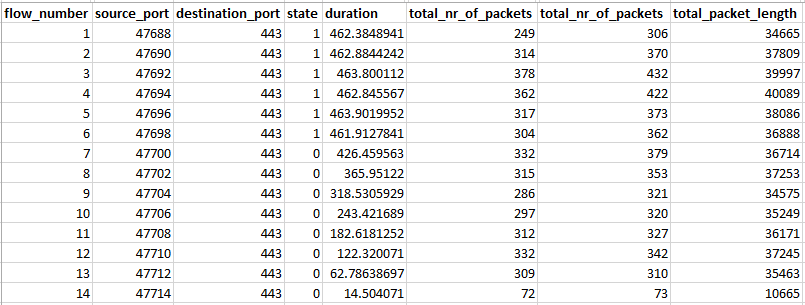
\includegraphics[scale=0.7]{images/eval_sg.PNG}
\centering
\caption{Summarized Evaluation of SecGrid}
\label{fig:sg}
\end{figure}

\begin{figure} [h]
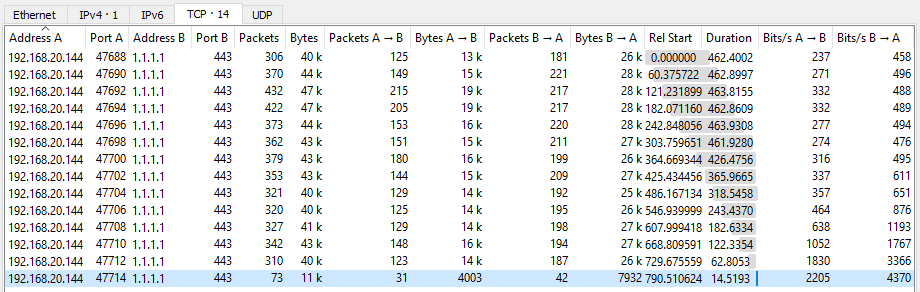
\includegraphics[scale=0.65]{images/eval_ws.PNG}
\centering
\caption{Summarized Evaluation of \textit{Wireshark}}
\label{fig:ws}
\end{figure}

\subsection{Comparison to Related Work} \label{comp_dohlyzer}
In this Section the result CSV file "\textit{doh\_brw\_mal\_iodine.pcap-ML-features-DoH.xlsx}" of SecGrid (Figure \ref{fig:sg}  and the result CSV file "\textit{doh\_brw\_mal\_iodine\_dohlyzer.xlsx}" computed with \cite{DoHlyzer} by \cite{montazerishatoori2020anomaly} (Figure \ref{fig:dohlyzer}). Considering the file computed with \cite{DoHlyzer}, the number of rows directly attracts the attention. There are totally 44 rows, i.e. 30 rows more than SecGrid. The rows contain the computed feature values of the different flows, whereas each flow is separated into small clumps limited by the timeout constant of probably 120 seconds. The timeout can be observed in the column \textit{duration}. Additionally, the clumps are separated into the direction of the flow, i.e. into requests from the client and responses from the server.

Since the clumps vary widely from the result file of SecGrid also the computed values of the clumps are very different and therefore they cannot be compared. But an interesting point is the number of rows in the file computed with \cite{DoHlyzer}, which is more than four times bigger than the number of rows in the file computed by SecGrid. This shows that the clumping process in SecGrid is more effective and memory saving than the one in \cite{DoHlyzer}. Also that the Feature Extraction module of SecGrid does not distinguish the flow direction can be seen as a clear strength, since \cite{BehnkeEtAl_FeatureEngineeringMLModelMaliciusDoHTraffic} removed the information about the IP addresses and the port information. It is possible that without this information the ML model has a deranging side noise, since it does not know from which side the data flow is coming. The Feature Extraction model of SecGrid bypasses this problem by summarizing the whole flow into one row and extracting the measures from it. Thus, the ML model cannot be disturbed by the flow direction anymore.

\begin{figure} [h]
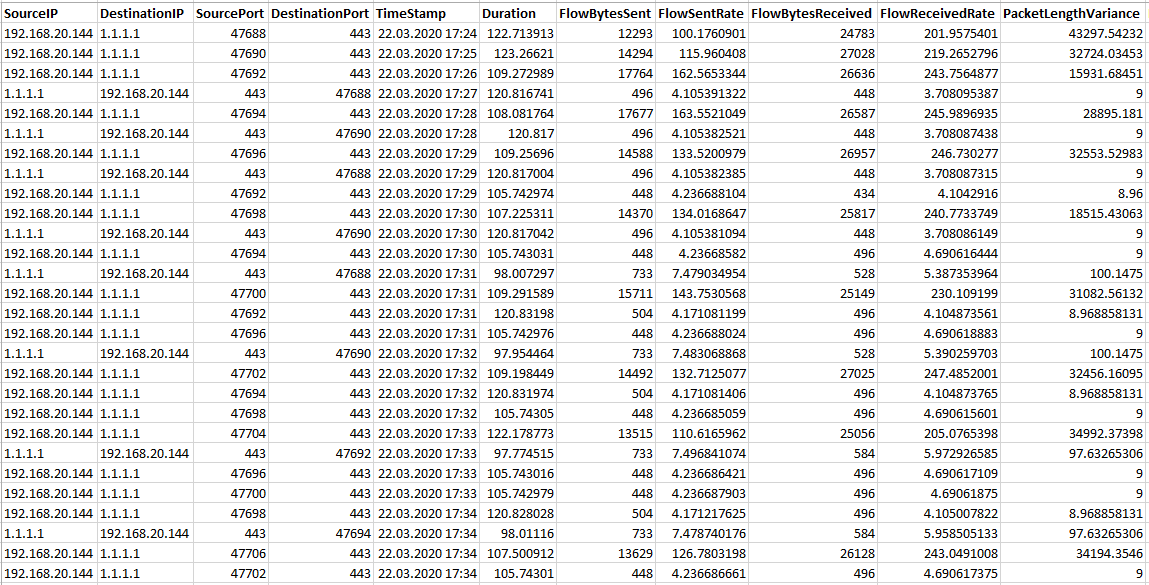
\includegraphics[scale=0.5]{images/example_dohlyzer.PNG}
\centering
\caption{Cutout from the summarized Evaluation of the DoHlyzer \cite{DoHlyzer} computed by \cite{montazerishatoori2020anomaly}}
\label{fig:dohlyzer}
\end{figure}

\section{Feature Importance}
In this Section, the relevance of the features that are adopted from \cite{montazerishatoori2020anomaly} and the novel features that are newly introduced in this thesis is discussed. The feature importance of tree based ML algorithms can be retrieved pretty simple in scikit-learn \cite{featureImportance}. As an output, a barplot is received where all the features are listed hierarchically according to their importance. The importance of a feature in a tree based ML algorithm means how many times the feature is needed for each tree that was built.

\subsection{Layer 1}
First the feature importance of Layer 1, which can be seen in Figure \ref{fig:feat_imp_l1} is discussed. \cite{BehnkeEtAl_FeatureEngineeringMLModelMaliciusDoHTraffic} found a feature sequence with descending order using statistical tests. This sequence is also used in this thesis. What attracts the attention at first is that compared to the feature importance in Figure \ref{fig:feature_importance} the feature importance that is found in Figure \ref{fig:feat_imp_l1} is not the same. There are definitely correlations, like the feature \textit{duration} or the feature \textit{response\_request\_mode} which are in the top segment of both figures, but there us also the feature \textit{flow\_bytes\_sent} which is situated in the middle of the hierarchy in Figure \ref{fig:feature_importance} but is in the second place in Figure \ref{fig:feat_imp_l1}. Also in the bottom section of both figures there are accordances and discordances. Regarding for example the feature \textit{packet\_length\_variation} which is situated in the bottom segment of both figures there can be found definitely accordances, but regarding the feature \textit{packet\_time\_standard\_deviation} there can also disaccordances be observed.

\begin{figure} [h]
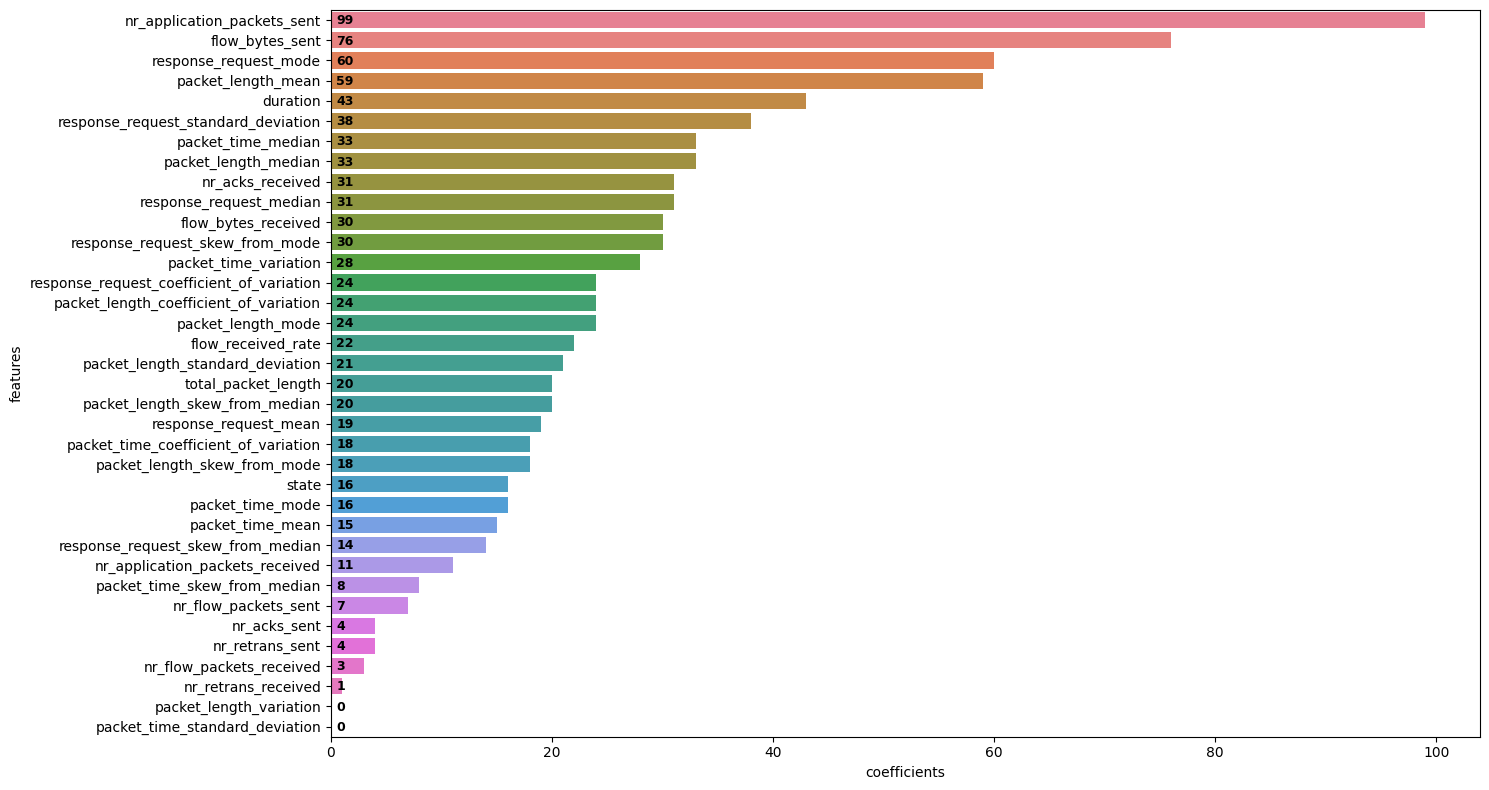
\includegraphics[scale=0.4]{images/feature_importance_layer_1.png}
\centering
\caption{Feature Importance of Layer 1}
\label{fig:feat_imp_l1}
\end{figure}

According to \cite{VeshkinEtAl_DoHInsightML}, the duration of a flow is one of the most important indicators to differentiate between DoH and non-DoH traffic. The evaluation in Figure \ref{fig:feat_imp_l1} confirms this statement, since the feature \textit{duration} is found in the top features of the most important ones of the model. Another very important indicator is the amount of data that is sent and received in a flow. This statement is validated as well, since the two features \textit{flow\_bytes\_sent} and \textit{flow\_bytes\_received} and also other features that indicated the amount of data sent in a flow can be found amongst the most important features of the model. Finally, the feature \textit{packet\_length\_mean} is found as the absolute most important feature. This finding is not surprising at all, since the size of the packet is also an important indicator for DoH and non-DoH traffic.

Some of the novel features that are introduced in this thesis do also have an impact on the model. At the head of the hierarchy the feature \textit{nr\_application\_packets\_sent}. This finding correlates with the statement of \cite{VeshkinEtAl_DoHInsightML}, who said that the amount of data sent in the flow is one of the most important differences between a normal HTTPS and a DoH connection. Thus, it is not surprising to find this feature as one of the most important ones. Another feature that can be found amongst the top of the most important features is the \textit{nr\_acks\_received}. This is not further surprising since if the number of packet sent is important, the number of ACKs also must have an impact on the model since received ACKs are the answer of the resolver that the packet was received. The feature \textit{total\_packet\_length} can be found in the middle of the hierarchy. It again correlates with the statement of \cite{VeshkinEtAl_DoHInsightML} that the amount of data sent in a flow is an important indicator for DoH or non-DoH traffic. The other features seem not to have a big impact to the model of Layer 1.

\subsection{Layer 2}
Second the feature importance of Layer 2, which is visualized in Figure \ref{fig:feat_imp_l2} is discussed. Compared to the feature sequence that \cite{BehnkeEtAl_FeatureEngineeringMLModelMaliciusDoHTraffic} found, the order is slightly different. On the one hand features like the \textit{duration} and the \textit{packet\_time\_skew\_from\_median} are found on top of the hierarchy in both sequences. On the other hand, features like \textit{packet\_length\_coefficient\_of\_variation} or \textit{flow\_received\_rate} are found on top of the sequence that \cite{BehnkeEtAl_FeatureEngineeringMLModelMaliciusDoHTraffic} found, but in the feature importance figure of Layer 2 they are found in the middle or in the lower part of the sequence. In reverse features like \textit{response\_request\_median} or \textit{flow\_bytes\_received} that are amongst the top of the most important features of the model of Layer 2 are situated in the middle or even in the bottom part of the sequence that \cite{BehnkeEtAl_FeatureEngineeringMLModelMaliciusDoHTraffic} found.

\begin{figure} [h]
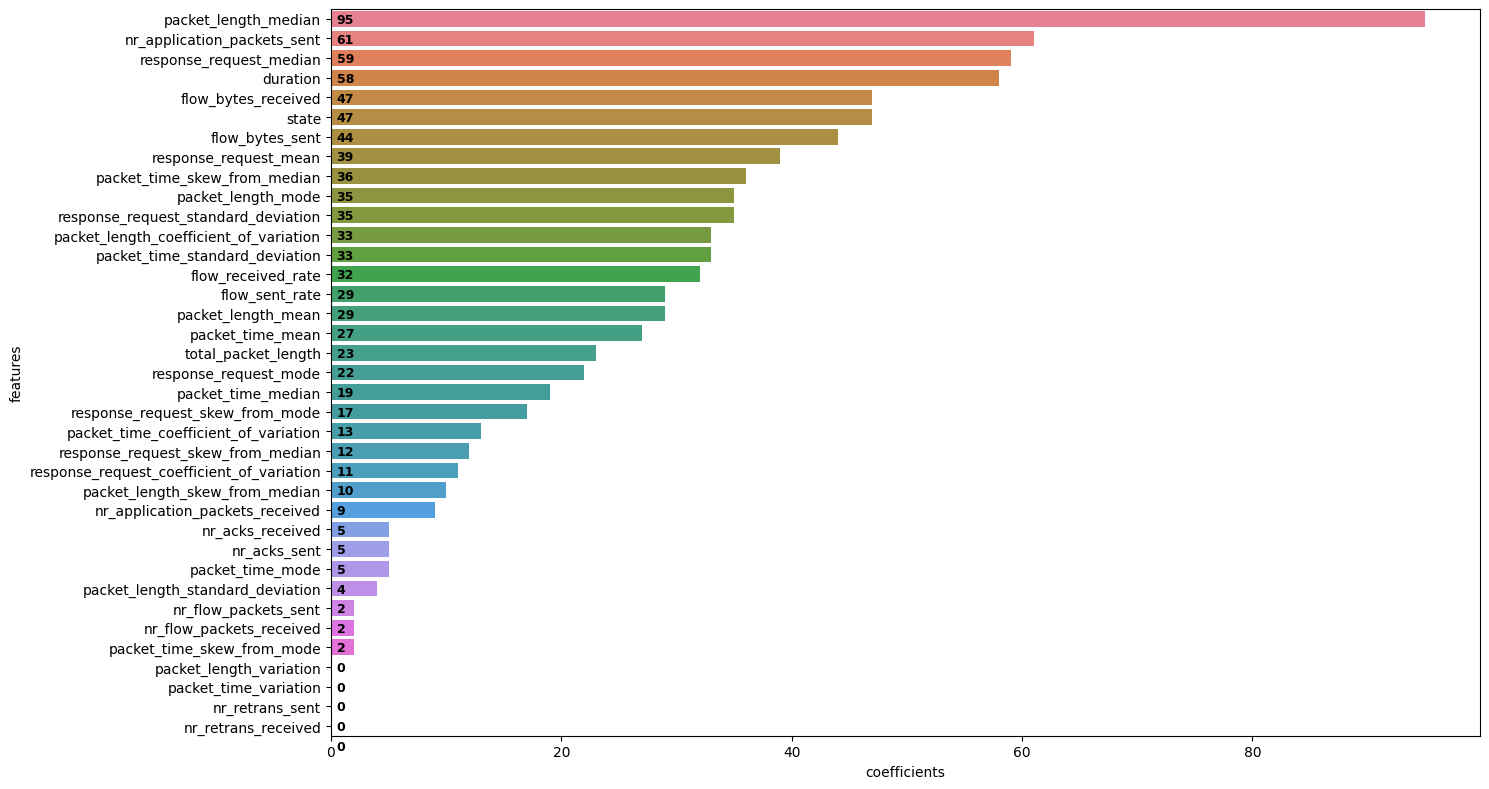
\includegraphics[scale=0.42]{images/feature_importance_layer_2.png}
\centering
\caption{Feature Importance of Layer 2}
\label{fig:feat_imp_l2}
\end{figure}

Figure \ref{fig:feat_imp_l2} shows additionally that some of the novel features have an impact on the model. The first feature found in the list is \textit{nr\_application\_packets\_sent}. Another feature that is found in the top of the hierarchy is the \textit{state}. It seems like either of the two traffic types is interrupted more than the other one. The feature \textit{total\_packet\_length} can be found in the middle of the hierarchy. The other features seem not to have a big impact to the model of Layer 2.

\subsection{Discussion}
The sequences \cite{BehnkeEtAl_FeatureEngineeringMLModelMaliciusDoHTraffic} seem to hold only partially. While there are in both Layers some correlations, there are also differences. The cognition is that the feature importance is slightly different for different ML models, which are trained with different training data-sets. Thus, it is important to keep all the features to train and test the ML model to not lose accuracy in the predictions of the ML model. 

An interesting finding of this thesis is that some the novel features seem to have an impact on the ML model and the consequential predictions. Especially the features \textit{nr\_application\_packets\_sent} and \textit{state} have to be highlighted. The \textit{nr\_application\_packets\_sent} can be found surprisingly on top of both of the evaluation figures of the two Layers. There seems to be a huge difference of the number of application packets sent between HTTPS connections and DoH connections as well as between benign and malicious DoH traffic. For malicious traffic this makes somehow sense, since the aim of malware is to exfiltrate data from the system of its victim in small slices to stay under the radar of warning systems. The other feature that needs to be highlighted is the \textit{state}. Especially in the hierarchy of Layer 2 it is found on the top. There seems to be a context between either benign or more likely malicious DoH traffic and non-ending TCP flows.

\section{ML Model}
In this Section, the ML models are evaluated. Before this can be done, all the metrics and figures that are used for this evaluation are presented. In a further step, the models of Layer 1 and Layer 2 are tested using all the presented metrics. Finally, to have a cross-validation the model of Layer 1 is tested using another data-set \cite{ieee_dataset}. Unfortunately, no other data-set that satisfy the requirements for Layer 2 could be found, therefore a cross-validation for Layer 2 is not possible.

\subsection{Metrics}
The evaluation of the ML models requires tautological metrics and figures, i.e. the performance, the accuracy, the recall, the precision, the F1-score, the specificity, the precision recall, and Receiver Operating Characteristics Curve (ROC). Therefore they are explained in this separate section and subsequently used for all the further ML evaluations.

\subsubsection{Performance}
On the basis of the findings of \cite{BehnkeEtAl_FeatureEngineeringMLModelMaliciusDoHTraffic}, the LGBM was newly implemented due to its alleged outstanding performance. In this thesis, the performance is the time which is needed to train the model and the time needed to classify one clump. During the implementation phase, the observation was made that the measured times are never exactly the same, they always deviate slightly from each other. Therefore the whole pipeline is run ten times and then the mean time is computed to ensure that an average performance time can be evaluated. Furthermore the Random Forest (RF) model which was already implemented into SecGrid was used to compare if the performance of the LGBM is indeed much better than the performance of RF, like \cite{BehnkeEtAl_FeatureEngineeringMLModelMaliciusDoHTraffic} stated.

\subsubsection{Confusion Matrix}
The confusion Matrix is a plot type that illustrates for the two classes 0 and 1 how many predictions for per class were successful and how many predictions were unsuccessful. It serves mainly to show the classification of the two classes since it is possible that they are not equally successful or unsuccessful classified. Figure \ref{fig:ex_conf_mat} shows the theoretic composition of a confusion matrix. If a data point was labeled as positive and predicted as positive, it is called a \textit{true positive} (TP). When a data-point is labeled as a positive but was predicted as a negative, it is called a \textit{false positive} (FP). Equally, when a data-point was labeled negative and was predicted negative, it is called a \textit{true negative} (TP), and when a data-point was labeled as negative but predicted as positive, it is called a \textit{false negative} (FN) \cite{Zheng2015EvaluatingML}. 

\begin{figure} [h]
    \centering
    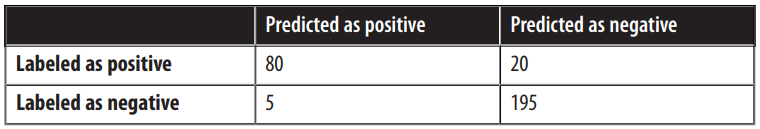
\includegraphics[scale=0.7]{images/ex_conf_mat.PNG}
    \caption{Theoretical Composition of a Confusion Matrix \cite{Zheng2015EvaluatingML}}
    \label{fig:ex_conf_mat}
\end{figure}

\subsubsection{Accuracy}
The accuracy of a ML Classifier indicates how often the model made the correct predictions compared to the total number of data to be predicted. Equation \ref{eq:accuracy} show how the accuracy is computed \cite{Zheng2015EvaluatingML}.

\begin{equation}
    accuracy = \frac{\# \; of \; correct \; Predictions}{\# \; of \; total \; Data \; Points}  = \frac{TP+TN}{TP+TN+FP+FN}
    \label{eq:accuracy}
\end{equation}

\subsubsection{Recall}
The recall of a ML Classifier indicates the percentage of the relevant elements found by the classifier out of the total amount of elements that are truly relevant. Therefore the amount of TP is divided by the sum of the TP and the FN, which can be seen in Equation \ref{eq:recall} \cite{Zheng2015EvaluatingML}.

\begin{equation}
    recall = \frac{TP}{TP+FN}
    \label{eq:recall}
\end{equation}

\subsubsection{Precision}
The precision of a ML Classifier indicates the percentage of the truly relevant elements out of the total amount of element predicted to be relevant. Therefore the amount to TP is divided by the sum of TP and FP, which can be seen in Equation \ref{eq:precision} \cite{Zheng2015EvaluatingML}.

\begin{equation}
    precision = \frac{TP}{TP+FP}
    \label{eq:precision}
\end{equation}

\subsubsection{F1-Score}
The F1-score or also the \textit{harmonic mean} and indicated the balance between the recall and the precision. It is  twice the product of the recall and the precision divided by the sum of the precision and the recall, which can be seen in Equation \ref{eq:f1-score} \cite{Zheng2015EvaluatingML}.

\begin{equation}
    F1-Score = 2*\frac{TP}{2TP+FN+FP}
    \label{eq:f1-score}
\end{equation}

\subsubsection{Receiver Operating Characteristics Curve}
The Receiver Operating Characteristics Curve (ROC curve) shows the rate of the amount of TP compared to the amount of TN classified by the model. In other words, it shows how many correct TPs and TNs are classified while the classification of FPs and FNs happens \cite{Zheng2015EvaluatingML}.

\subsection{Layer 1 using Data-Set CIRA-CIC-DoHBrw-2020} \label{eval_l1}
For the evaluation of Layer 1 a special testing data-set was created. It contains 4000 equally distributed clumps, i.e. 2000 non-DoH traffic data and 2000 DoH traffic data. Since there is not enough benign DoH data available in the data-set \cite{CIRA-CIC-DoHBrw-2020}, benign DoH data from TSL2 is taken to ensure that not the same data from TSL1 is tested and to complement 1000 clumps. The exact distribution can be seen in Table \ref{tab:tds_l1}. 

\begin{center}
\begin{longtable}{ |l|l|c|c|c|c| }
\hline
\multicolumn{2}{|c|}{ } & \makecell{Non-DoH\\(Chrome)} & \makecell{Non-DoH\\(Firefox)} & \makecell{DoH\\(Chrome)} & \makecell{DoH\\(Forefox)} \\
\hline
\multirow{4}{*}{Benign}
& AdGuard & 250 & 250 & 25 & 125 \\
& Cloudflare & 250 & 250 & 45 & 125 \\
& Google & 250 & 250 & 90 & 125 \\
& Quad9 & 250 & 250 & 340 & 125 \\
\hline
\multirow{3}{*}{Malicious}
& DNS2TCP & \multicolumn{2}{|c|}{0} & \multicolumn{2}{|c|}{4000}  \\
& DNScat2 & \multicolumn{2}{|c|}{0} & \multicolumn{2}{|c|}{3000} \\
& iodine & \multicolumn{2}{|c|}{0} & \multicolumn{2}{|c|}{3000} \\
\hline
\multicolumn{2}{|l|}{Total} & \multicolumn{2}{|c|}{2000} & \multicolumn{2}{|c|}{2000} \\
\hline
\caption{Distribution of the Data-Points in TSL1}
\label{tab:tds_l1}
\end{longtable}
\end{center}

\subsubsection{Performance}
The mean duration of the training of Layer 1 is 3.57 seconds, the prediction duration of Layer 1 is 0.04 Seconds, using 39 features. \cite{BehnkeEtAl_FeatureEngineeringMLModelMaliciusDoHTraffic} stated that with the default hyperparameters their model needed totally 87 seconds for the whole process of Layer 1, using 21 features.

\subsubsection{Accuracy \& Confusion Matrix}
The accuracy of Layer 1 is 0.9855. Compared to \cite{BehnkeEtAl_FeatureEngineeringMLModelMaliciusDoHTraffic}, who received an accuracy of 0.9978 it is slightly inferior, but it is still a good result. The confusion matrix of Layer 1 can be seen in Figure \ref{fig:con_roc_l1} on the left. It shows in each case out of 2000 clumps only seven non DoH traffic clumps are not classified correctly, whereas 51 DoH traffic columps are not classified correctly.

\begin{figure*}[ht]
\centering
\subfloat{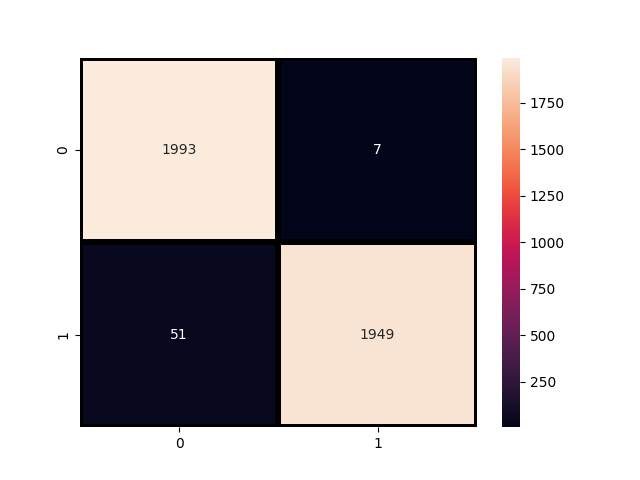
\includegraphics[width=0.45\textwidth]{images/confusion_matrix_layer_1.png}}\hspace{1.0cm}
\subfloat{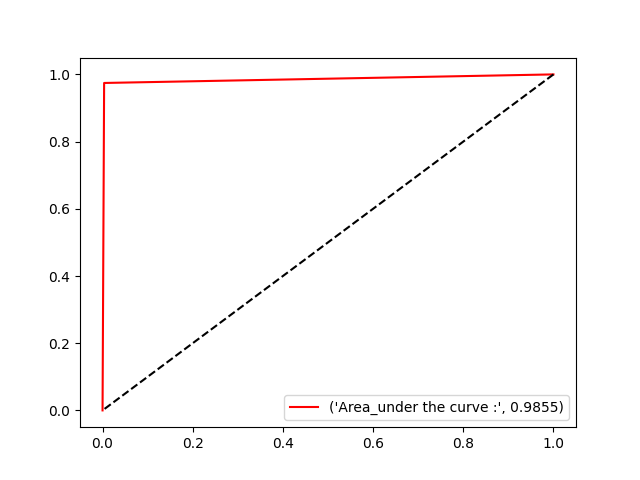
\includegraphics[width=0.45\textwidth]{images/roc_curve_layer1.png}}
\caption{Confusion Matrix (left) and ROC Curve of (right) of Layer 1}
\label{fig:con_roc_l1}
\end{figure*}

\subsubsection{Recall, Precision, F1-Score \& ROC Curve}
The recall for the non DoH traffic part is 1.00, the recall for the DoH traffic part is 0.97, which results in an average recall of 0.985. The precision for the non DoH traffic part is 0.98, the recall for the DoH traffic part is 1.00, which results in an average recall of 0.99. The f1-score for the non DoH traffic part is 0.99, the recall for the DoH traffic part is 0.99, which results in an average recall of 0.99. Table \ref{tab:rpf1l1} shows an overview of the computed values. Since the amount of non-DoH clumps and the amount of DoH clumps is equal, also the macro average and the wieghted average are equal, therefore only the superficial term "average" is used here. The ROC Curve of Layer 1 can be seen in Figure \ref{fig:con_roc_l1} on the right. Again, it shows the accuracy of the model and makes certain that nearly every data-point is classified correctly, with an insignificant part of FPs and FNs.

\begin{center}
\begin{longtable}{ |l|c|c|c| }
\hline
 & Recall & Precision & F1-Score \\
\hline
non-Doh & 1.00 & 0.98 & 0.99 \\
\hline
DoH & 0.97 & 1.00 & 0.99 \\
\hline
Average & 0.985 & 0.99 & 0.99 \\ 
\hline
\end{longtable}
\captionof{table}{Recall, Prescison and F1-Score of Layer 1}
\label{tab:rpf1l1}
\end{center}

\subsubsection{Discussion}
As already mentioned before, the accuracy of \cite{BehnkeEtAl_FeatureEngineeringMLModelMaliciusDoHTraffic} is not quite reached, but the results are still excellent. Also the precision, the recall and the f1-score are exceptional. Concerning the performance, the model which was implemented into SecGrid is massively faster than the model of \cite{BehnkeEtAl_FeatureEngineeringMLModelMaliciusDoHTraffic}, although they used only 21 features unlike the model in SecGrid which uses 39 features. The prediction time, which lasted 0.04 seconds is sensational and suits excellently for a system like SecGrid that promises fast detection times.

\subsection{Layer 2 using Data-Set CIRA-CIC-DoHBrw-2020} \label{eval_l2}
Similar to the evaluation of Layer 1 a special test data-set is compiled. It contains 4000 data-points which are equally distributed to 2000 benign DoH clumps and 2000 malicious DoH clumps. Again, since not enough benign DoH clumps are available, benign DoH clumps from TSL1 are taken to ensure that the test data-set contains 2000 benign DoH clumps and that not data from TSL2 is taken. The exact distribution of this test data-set is presented in Table \ref{tab:tds_l2}.

\begin{center}
\begin{longtable}{ |l|c|c|c|c| }
\hline
 & \makecell{Benign\\(Chrome)} & \makecell{Benign\\(Firefox)} & Malicious \\
\hline
AdGuard & 25 & 250 & 0 \\
Cloudflare & 45 & 250 & 0 \\
Google & 90 & 250 & 0 \\
Quad9 & 840 & 250 & 0 \\
\hline
DNS2TCP & \multicolumn{2}{|c|}{0} & 800 \\
DNScat2 & \multicolumn{2}{|c|}{0} & 600 \\
iodine & \multicolumn{2}{|c|}{0} & 600 \\
\hline
Total & \multicolumn{2}{|c|}{2000} & 2000 \\
\hline
\caption{Distribution of the Data-Points in TSL2}
\label{tab:tds_l2}
\end{longtable}
\end{center}

\subsubsection{Performance}
The mean duration of the training Layer 2 is 4.18 seconds, the mean predicting duration is 0.084 seconds using 37 features. \cite{BehnkeEtAl_FeatureEngineeringMLModelMaliciusDoHTraffic}'s approach had a total duration of 40 seconds for the training and the prediction phase of Layer 2 using 27 features.

\subsubsection{Accuracy \& Confusion Matrix}
The accuracy of Layer 2 is 0.99975. Compared to \cite{BehnkeEtAl_FeatureEngineeringMLModelMaliciusDoHTraffic} who received an accuracy of 0.99996 it is again slightly inferior, but it is still a good result. Figure \ref{fig:con_roc_l2} on the left shows the confusion matrix of Layer 2. It depicts that only one benign DoH traffic clump is wrong classified, the malicious DoH traffic clumps were all correctly predicted.

\begin{figure*}[ht]
\centering
\subfloat{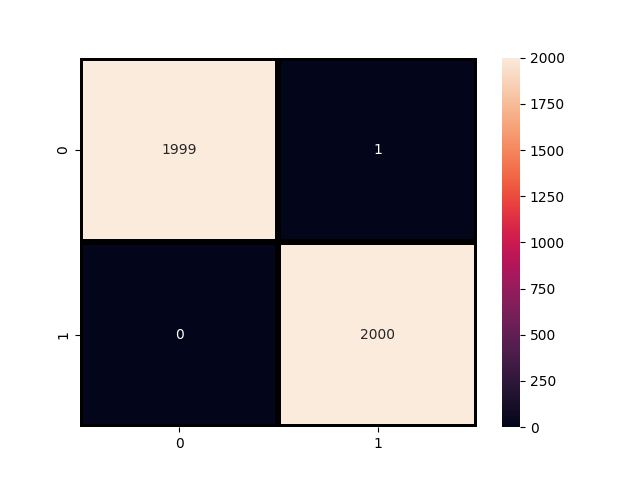
\includegraphics[width=0.45\textwidth]{images/confusion_matrix_layer_2.png}}\hspace{1.0cm}
\subfloat{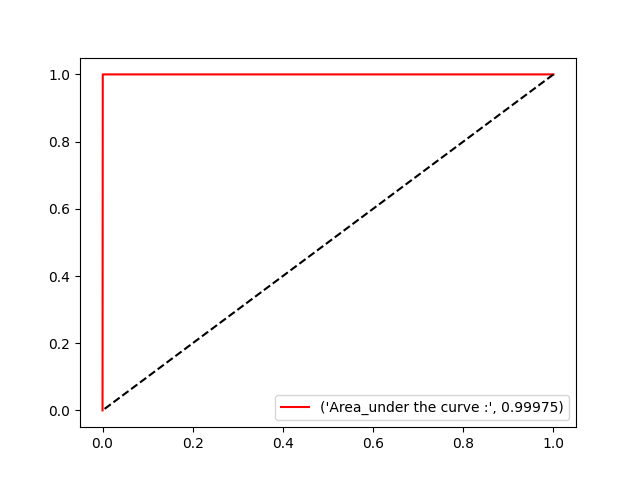
\includegraphics[width=0.45\textwidth]{images/roc_curve_layer2.png}}
\caption{Confusion Matrix (left) and ROC Curve of (right) of Layer 2}
\label{fig:con_roc_l2}
\end{figure*}

\subsubsection{Recall, Precision, F1-Score \& ROC Curve}
The averages of recall, the precision and the f1-score are all 1.0. This means that for each of the three metrics the benign DoH traffic as well as the malicious DoH traffic was computed to 1.0. They are all listed in Table \ref{tab:rpf1l2}. The ROC Curve of Layer 2 can be seen in Figure \ref{fig:con_roc_l2} on the right. It reinforces again how precise the model is, since the angle in the top left corner is nearly 90° which means that there is only one FN and no FPs.

\begin{center}
\begin{longtable}{ |l|c|c|c| }
\hline
 & Recall & Precision & F1-Score \\
\hline
non-Doh & 1.00 & 1.0 & 1.0 \\
\hline
DoH & 1.0 & 1.00 & 1.0 \\
\hline
Average & 1.0 & 1.0 & 1.0 \\ 
\hline
\end{longtable}
\captionof{table}{Recall, Precising and F1-Score of Layer 1}
\label{tab:rpf1l2}
\end{center}

\subsubsection{Discussion}
As already mentioned before, the accuracy of \cite{BehnkeEtAl_FeatureEngineeringMLModelMaliciusDoHTraffic} is not quite reached, but like already in the first Layer, the results are still excellent. The computed values for the precision, the recall and the f1-score is outstanding and cannot be better. It means that the model is able to predict nearly every malicious clump extracted from the data-set \cite{CIRA-CIC-DoHBrw-2020} correctly. Concerning the performance of the model implemented into SecGrid, it is massively faster than the model of \cite{BehnkeEtAl_FeatureEngineeringMLModelMaliciusDoHTraffic}. With a prediction time of 0.084 seconds, the model is extremely fast, which is perfect for a system like SecGrid that relies on fast results. Summarized, the whole pipeline delivers astonishing results while using the data-set \cite{CIRA-CIC-DoHBrw-2020}.

\subsection{Performance using Random Forest Algorithm}
\cite{BehnkeEtAl_FeatureEngineeringMLModelMaliciusDoHTraffic} found that the LGBM algorithm is much faster than the Random Forest (RF) algorithm. This intention of this section is to verify this statement. Therefore instead of the LGBM, the RF is implemented. To do so, there are only three lines to be changed in the code: the import of LGBM has to be changed to the import of RF and the two lines where LGBM is initiated have to be changed to the initiation of RF. Since \cite{BehnkeEtAl_FeatureEngineeringMLModelMaliciusDoHTraffic} used the default modulations of RF, they are also used for the verification in this work.

Like in Sections \ref{eval_l1} and \ref{eval_l2}, the whole pipeline is run ten times, the durations of the training phases of both Layers and the durations of the predictions phases of both layers are measured. Then, the mean duration of all the four different durations is computed. The training phase of Layer 1 lased 17.74 seconds, the prediction phase of Layer 1 lasted 0.036 seconds. Thus, RF needs more than four times as much time than LGBM needs for the training Layer 1, whereas the duration of prediction phase is slightly smaller. The training phase of Layer 2 lasted 14.94 seconds and the prediction phase of Layer 1 lasted 0.060 seconds. Thus RF needs more than twice as much time as LGBM for the training phase, whereas the prediction time of RF is slightly smaller.

The finding of this Section is that the LGBM algorithm was a good choice concerning the performance. Although the RF algorithm is slightly faster in predicting, it is in return extremely slower in predicting. However, it cannot be negligible that no hyperparameter optimization was conducted for the RF algorithm. Comparing the results with \cite{BehnkeEtAl_FeatureEngineeringMLModelMaliciusDoHTraffic}, it is conspicuous that their model of of Layer 1 needed 4991 seconds and the model of Layer 2 needed 890 seconds for the whole process. 

\section{Layer 1 using a Different Data-set}
Since the results of Layer 1 and are truly impressive, the aim of this Section is to validate these good results. The original plan was to take a data-set that contains traffic for both Layers, but unfortunately \cite{CIRA-CIC-DoHBrw-2020} is the only available data-set that contains malicious DoH traffic. Therefore only Layer 1 can be tested with other traffic data. To this end, a second data-set taken from the IEEE Dataport \cite{ieee_dataset} is introduced. This data-set contains DoH and non-DoH traffic collected by using the two Browsers Chrome and Firefox. In addition, the two data-sets were generated by using different modulations and towards multiple DoH resolvers. The list of the IP-addresses of the DoH resolvers can be found in Table \ref{tab:doh_ips_ieee}. It is conspicuous that they used partially the same DoH resolvers, but also other DoH resolvers that \cite{CIRA-CIC-DoHBrw-2020} did not use. Furthermore, the amount of DoH resolvers used is bigger in \cite{ieee_dataset} than in \cite{CIRA-CIC-DoHBrw-2020}. All these differences are good for the validation with other data than the original data-set because it is an ultimate test to see if the system can handle also data from outside the lab-generated data-set \cite{CIRA-CIC-DoHBrw-2020}.

\begin{center}
\begin{longtable}{ |c|c|c| }
\hline
\multicolumn{3}{|c|}{DoH Resolver IP-Address} \\
\hline
88.198.91.187 & 88.198.91.187 & 104.22.72.65 \\
\hline
104.16.249.249 & 104.16.248.249 & 104.22.73.65 \\
\hline
104.16.249.249 & 104.16.248.249 & 176.9.1.117 \\
\hline
146.112.41.2 & 146.112.41.3 & 176.9.93.198\\
\hline
185.43.135.1 & 185.235.81.1 & 5.1.66.255\\
\hline
104.236.178.232 & 195.30.94.28 & 159.69.198.101\\
\hline
\caption{IP-Addresses of the DoH Resolvers used for the Data-Set \cite{ieee_dataset}}
\end{longtable}
\label{tab:doh_ips_ieee}
\end{center}

\subsection{Preprocessing} \label{ieee_preproc}
The data-set has to be preprocessed like the former data-set. Therefore, the two folders with one containing the traffic data that was collected using Chrome and the other one containing the data that was collected using Firefox is analyzed with the \textit{Feature Extraction} component of SecGrid. To differentiate between non-DoH and DoH traffic, the IP addresses introduced in table \ref{tab:doh_ips_ieee} are used. The analysis ended up in four different CSV files, i.e. clumps of Chrome non-DoH traffic, Chrome DoH traffic, Firefox non-DoH traffic and Firefox DoH traffic.

\subsection{\cite{ieee_dataset} as Test-Dataset} \label{ieee_as_testing_ds}
For the execution of this examination a test data-set has to be created. This test data-set contains 4000 equally distributed clumps from all the four referred CSV files in Section \ref{ieee_preproc}. This means that each from each of the CSV files 1000 random data-points are collected and saved into a new file called \textit{IEEETestDataset}. This test data-set is then saved as \textit{IEEETestDataset.csv} and used as the prediction data-set of Layer 1. Following the results of this test are presented.

\subsubsection{Accuracy \& Confusion Matrix}
The accuracy of Layer 1 using the data-set \cite{ieee_dataset} as testing is 0.6255. The confusion Matrix in Figure \ref{fig:con_roc_l1_i3e_test} on the left shows that the non-DoH clumps are predicted mostly correct with a negligible amount of 70 clumps which were predicted incorrect. But looking at the DoH clumps the confusion matrix unveils that only about 30\% are predicted correctly. This is a poor result, since the primary task of this Layer is to classify the clumps correctly into DoH and non-DoH clumps for the further processing in Layer 2.

\begin{figure*}[ht]
\centering
\subfloat{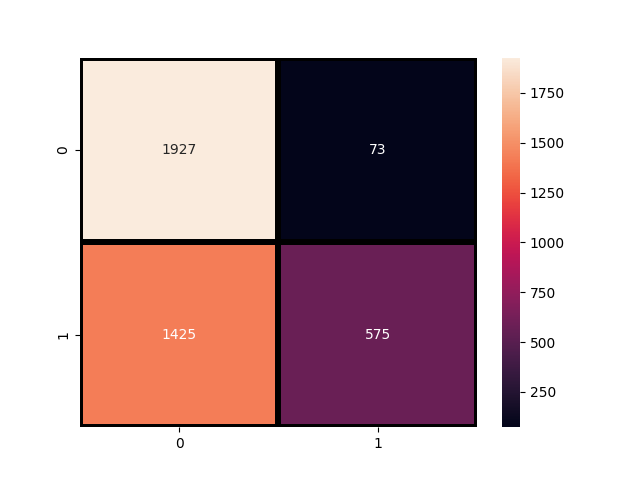
\includegraphics[width=0.45\textwidth]{images/confusion_matrix_layer_1_ieee_dataset.png}}\hspace{1.0cm}
\subfloat{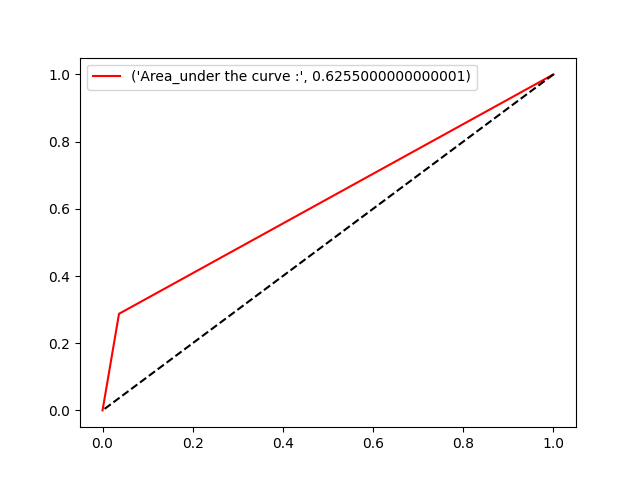
\includegraphics[width=0.45\textwidth]{images/roc_curve_layer1_ieee_dataset.png}}
\caption{Confusion Matrix (left) and ROC Curve of (right) of Layer 1 using Data from \cite{ieee_dataset} as Testing Data-Set}
\label{fig:con_roc_l1_i3e_test}
\end{figure*}

\subsubsection{Recall, Precision, F1-Score \& ROC Curve}
The average recall of Layer 1 using data of the data-set \cite{ieee_dataset} as prediction data is 0.63, the average precision is 0.73 and the average f1-score is 0.58. All the values can be seen in Table \ref{tab:rpf1l1_i3e_testds}. Figure \ref{fig:con_roc_l1_i3e_test} on the right shows the ROC-curve, which reinforces the inaccuracy of Layer 1.

\begin{center}
\begin{longtable}{ |l|c|c|c| }
\hline
 & Recall & Precision & F1-Score \\
\hline
non-Doh & 0.96 & 0.57 & 0.72 \\
\hline
DoH & 0.29 & 0.89 & 0.43 \\
\hline
Average & 0.63 & 0.73 & 0.58 \\ 
\hline
\end{longtable}
\captionof{table}{Recall, Precision and F1-Score of Layer 1 using Data of \cite{ieee_dataset} for the Test Data-Set}
\label{tab:rpf1l1_i3e_testds}
\end{center}

\subsubsection{Discussion}
This examination showed that the newly implemented model has difficulties to handle other data than data from the data-set \cite{CIRA-CIC-DoHBrw-2020}. On the one hand, the model is highly accurate in predicting non-DoH data, but on the other hand only about 30\% of the DoH data was predicted correctly. This contradicts the findings of Sections \ref{eval_l1} and \ref{eval_l2}, where it is proven that the model is very accurate. It seems that Layer 1 is able to separate data from the original data-set, but as soon as other data is involved it is not accurate anymore.

\subsection{Exclusively Data from \cite{ieee_dataset}} \label{exclusive_data}
The findings of Section \ref{ieee_as_testing_ds} are humbling. Thus, in this Section the data-set \cite{ieee_dataset} is tested if it is generally suited for the separation of non-DoH and DoH traffic. Therefore a training data-set of the same size as the original training data-set is created, i.e. it contains 40'000 clumps. These 40'000 are divided in half, whereas the first half contains 10'000 clumps non-DoH traffic collected using Chrome and 10'000 non-DoH clumps collected using Firefox. The other half contains 10'000 clumps of DoH traffic collected with Chrome and 10'000 clumps of DoH traffic collected using Firefox. This data-set is the saved in the CSV file called \textit{TSL1IEEE.csv}. This training data-set is now used to train Layer 1 and after the training it is tested with the testing set \textit{IEEETestDataset.csv}.

\subsubsection{Accuracy \& Confusion Matrix}
The accuracy of Layer 1 is using the data-set \cite{ieee_dataset} as training and testing set is 0.9885. The confusion matrix in Figure \ref{fig:con_roc_l1_i3e_train_test} on the left reveals that the non-DoH traffic clumps as well as the DoH traffic clumps are predicted predominantly correct. Only 32 non-DoH traffic clumps and 14 DoH traffic clumps are predicted incorrectly, thus those numbers are negligible. This is a excellent result which already indicates that the data-set is in principle eligible as training data-set for Layer 1.

\begin{figure*}[ht]
\centering
\subfloat{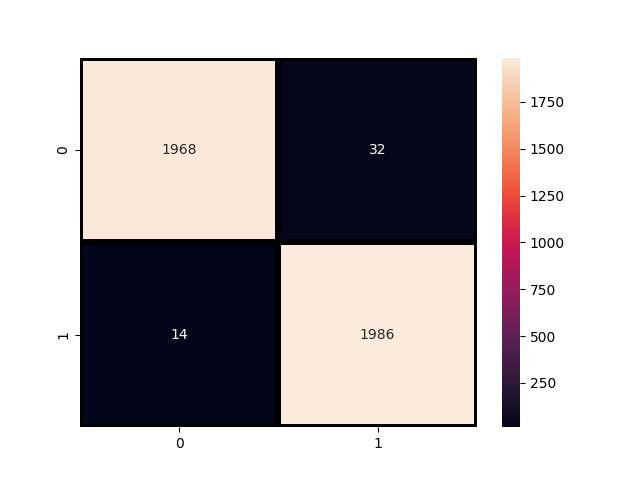
\includegraphics[width=0.45\textwidth]{images/confusion_matrix_layer_1_ieee_dataset_train_test.png}}\hspace{1.0cm}
\subfloat{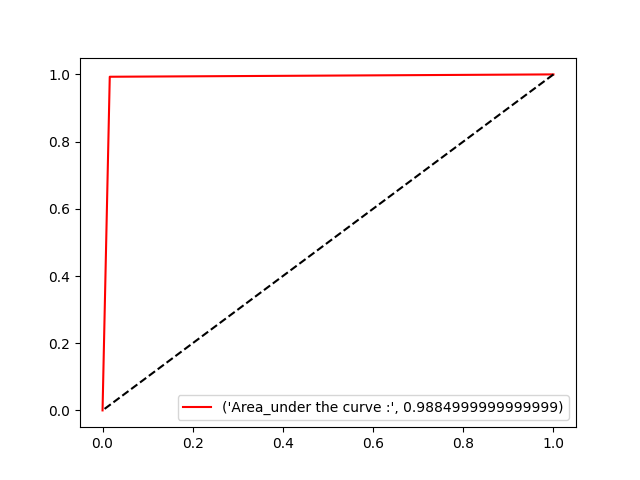
\includegraphics[width=0.45\textwidth]{images/roc_curve_layer1_ieee_dataset_train_test.png}}
\caption{Confusion Matrix (left) and ROC Curve of (right) of Layer 1 using Data from \cite{ieee_dataset} Training- and Testing Data-Set}
\label{fig:con_roc_l1_i3e_train_test}
\end{figure*}

\subsubsection{Recall, Precision, F1-Score \& ROC Curve}
The average recall of Layer 1 using data from \cite{ieee_dataset} as training and testing data-set is 0.99, the average precision is 0.99 and the average F1-score is 0.99. Table \ref{tab:rpf1l1_i3e_train_testds} shows that only the recall of the prediction of non-DoH traffic clumps and the precision of the prediction of DoH traffic clumps is 0.98, all the residual values are 0.99. The ROC curve in Figure \ref{fig:con_roc_l1_i3e_train_test} reinforces that the model is exact and that there are nearly no miss-predictions in the model.

\begin{center}
\begin{longtable}{ |l|c|c|c| }
\hline
 & Recall & Precision & F1-Score \\
\hline
non-Doh & 0.98 & 0.99 & 0.99 \\
\hline
DoH & 0.99 & 0.98 & 0.99 \\
\hline
Average & 0.99 & 0.99 & 0.99 \\ 
\hline
\end{longtable}
\captionof{table}{Recall, Precision and F1-Score of Layer 1 using Data of \cite{ieee_dataset} for the Training and the Test Data-Set}
\label{tab:rpf1l1_i3e_train_testds}
\end{center}

\subsubsection{Discussion}
This experiment shows that if the DoH detection component of SecGrid is applied to data that comes from the same data-set is highly accurate with an accuracy of 98.85\%. Only a negligible part of both, non-DoH traffic clumps and DoH traffic clumps is predicted wrong. Additionally, the viability of the data-set \cite{ieee_dataset} is proven when the training and the testing data-set come from it. This means that the DoH detection component of Layer 1 is basically exact, but it cannot be applied to detect DoH traffic from the dataset \cite{ieee_dataset} while it is trained with data from the data-set \cite{CIRA-CIC-DoHBrw-2020}.

\subsection{\cite{ieee_dataset} as Training Data-Set}
The last experiment of this Chapter is to test if the data of \cite{CIRA-CIC-DoHBrw-2020} is better predictable using data from \cite{ieee_dataset} as training data. To do so the same training data-set is used as in Section \ref{exclusive_data}. As the testing data-set, the same data-set is used as in Section \ref{eval_l1}.

\subsubsection{Accuracy \& Confusion Matrix}
The accuracy of Layer 1 using data from the data-set \cite{ieee_dataset} as training data-set and the test data from the data-set \cite{CIRA-CIC-DoHBrw-2020} is 0.7235. The confusion matrix in Figure \ref{fig:con_roc_l1_i3e_trainds} reveals that the non-DoH traffic clumps are predicted nearly perfectly. But as already experienced in Section \ref{ieee_as_testing_ds}, the prediction of the DoH traffic clumps is not good. With nearly 50\% correct predictions it was at least not as poor as the experiment result in Section \ref{ieee_as_testing_ds}, but this result is still not good.

\begin{figure*}[ht]
\centering
\subfloat{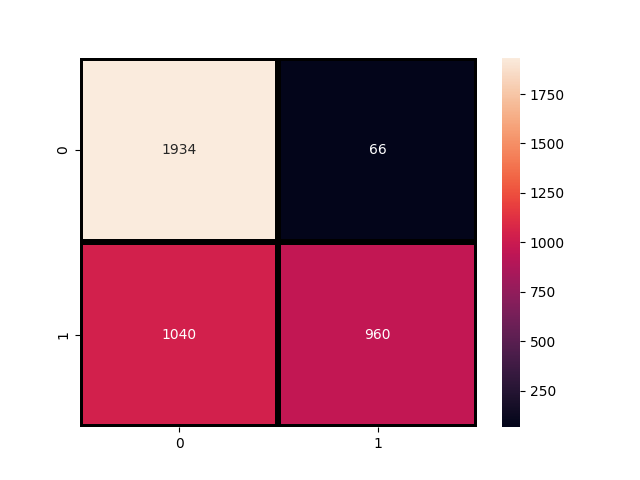
\includegraphics[width=0.45\textwidth]{images/confusion_matrix_layer_1_ieee_training_dataset.png}}\hspace{1.0cm}
\subfloat{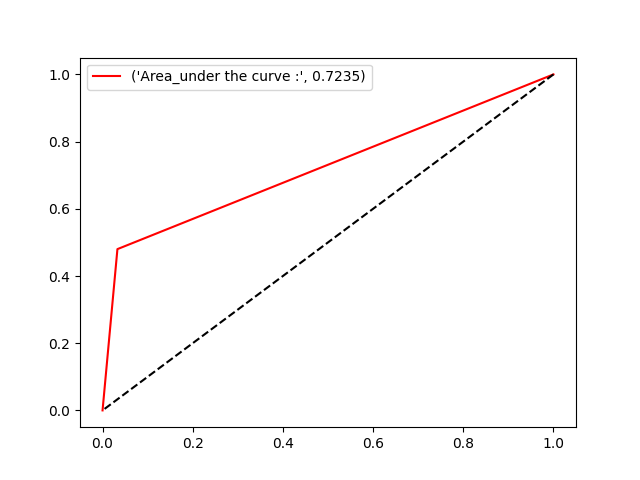
\includegraphics[width=0.45\textwidth]{images/roc_curve_layer1_ieee_training_dataset.png}}
\caption{Confusion Matrix (left) and ROC Curve of (right) of Layer 1 using Data from \cite{ieee_dataset} as Testing Data-Set}
\label{fig:con_roc_l1_i3e_trainds}
\end{figure*}

\subsubsection{Recall, Precision, F1-Score \& ROC Curve}
The average recall of Layer 1 using data from \cite{ieee_dataset} as training data-set and the test data from the data-set \cite{CIRA-CIC-DoHBrw-2020} is 0.72, the average precision is 0.79, and the average F1-score is 0.71. Table \ref{tab:rpf1l1_i3e_trainds} shows that especially the recall of the prediction of the DoH traffic clumps is poor since it is under 50\%. Figure \ref{fig:con_roc_l1_i3e_trainds} clarifies that the performance of this model is also not sufficient.

\begin{center}
\begin{longtable}{ |l|c|c|c| }
\hline
 & Recall & Precision & F1-Score \\
\hline
non-Doh & 0.97 & 0.65 & 0.78 \\
\hline
DoH & 0.48 & 0.94 & 0.63 \\
\hline
Average & 0.72 & 0.79 & 0.71 \\ 
\hline
\end{longtable}
\captionof{table}{Recall, Precision and F1-Score of Layer 1 using Data of \cite{ieee_dataset} for the Training Data-Set}
\label{tab:rpf1l1_i3e_trainds}
\end{center}

\subsubsection{Discussion}
This experiment shows again that the two different data-sets are not compatible to each other. Although the accuracy with 72.35\% was about 10\% higher than the result of the experiment in Section \ref{ieee_as_testing_ds}, this is still not the desired performance. The awareness that can be gained from this experiment is that the different browser settings and the different DoH-servers that were used to generate the data-set \cite{ieee_dataset} disturb in some manner the model when it is trained with data from the data-set \cite{CIRA-CIC-DoHBrw-2020}.
